\subsection{Rare and forbidden decays}
\label{sec:charm:rare}

This section provides a summary of rare and forbidden charm decays
in tabular form. The decay modes can be categorized as 
flavor-changing neutral currents, lepton-flavor-violating, 
lepton-number-violating, and both baryon- and lepton-number-violating decays.
Figures~\ref{fig:charm:rare_d0}-\ref{fig:charm:lambdac} plot the 
upper limits for $D^0$, $D^+$, $D_s^+$, and $\Lambda_c^+$ decays. 
Tables~\ref{tab:charm:rare_d0}-\ref{tab:charm:rare_lambdac} give the 
corresponding numerical results. Some theoretical predictions are given in 
Refs.~\cite{Burdman:2001tf,Fajfer:2002bu,Fajfer:2007dy,Golowich:2009ii,Paul:2010pq,Borisov:2011aa}.

In several cases the rare-decay final states have been observed with the di-lepton pair being the decay product of a hadronic resonance.
For these measurements the quoted limits are those expected for the non-resonant di-lepton spectrum.
For the extrapolation to the full spectrum a phase-space distribution of the non-resonant component has been assumed.
This applies to the CLEO measurement of the decays $D_{(s)}^+\to(K^+\pi^+)e^+e^-$~\cite{Rubin:2010cq}, to the D0 measurements of the decays $D_{(s)}^+\to\pi^+\mu^+\mu^-$~\cite{Abazov:2007aj}, and to the \babar measurements of the decays $D_{(s)}^+\to(K^+\pi^+)e^+e^-$ and $D_{(s)}^+\to(K^+\pi^+)\mu^+\mu^-$, where the contribution from $\phi\to l^+l^-$ ($l=e,\mu$) has been excluded.
In the case of the LHCb measurements of the decays $D^0\to\pi^+\pi^-\mu^+\mu^-$~\cite{Aaij:2013uoa} as well as the decays $D_{(s)}^+\to\pi^+\mu^+\mu^-$~\cite{Aaij:2013sua} the contributions from $\phi\to l^+l^-$ as well as from $\rho,\omega\to l^+l^-$ ($l=e,\mu$) have been excluded. 

\begin{figure}
\begin{center}
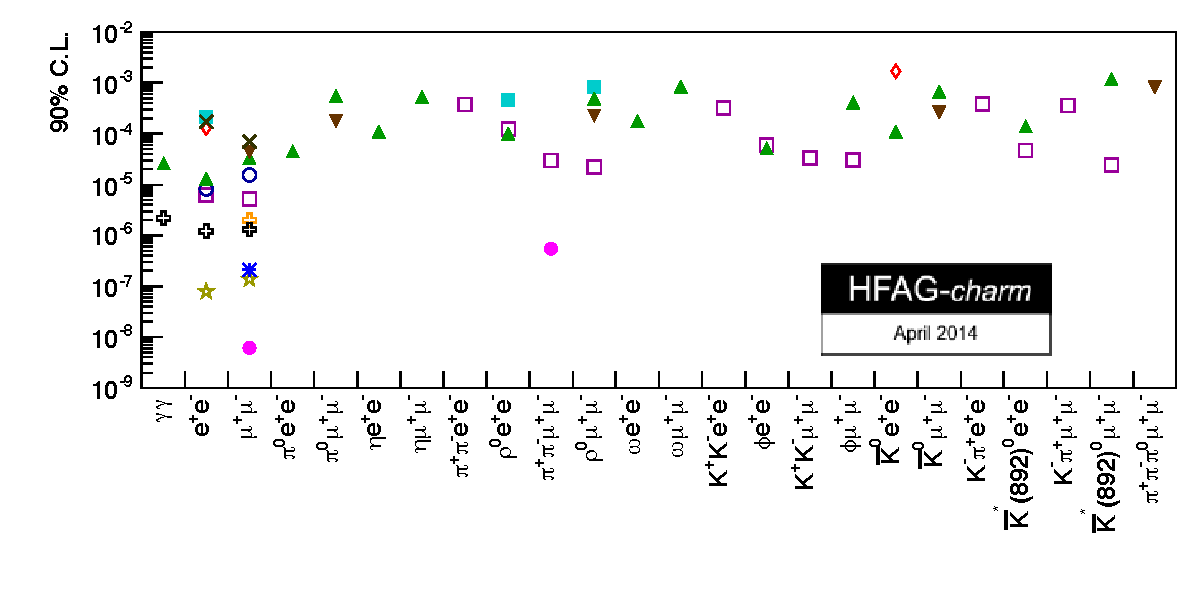
\includegraphics[width=6.0in]{figures/charm/rare_D0_1.pdf}
\vskip-0.10in
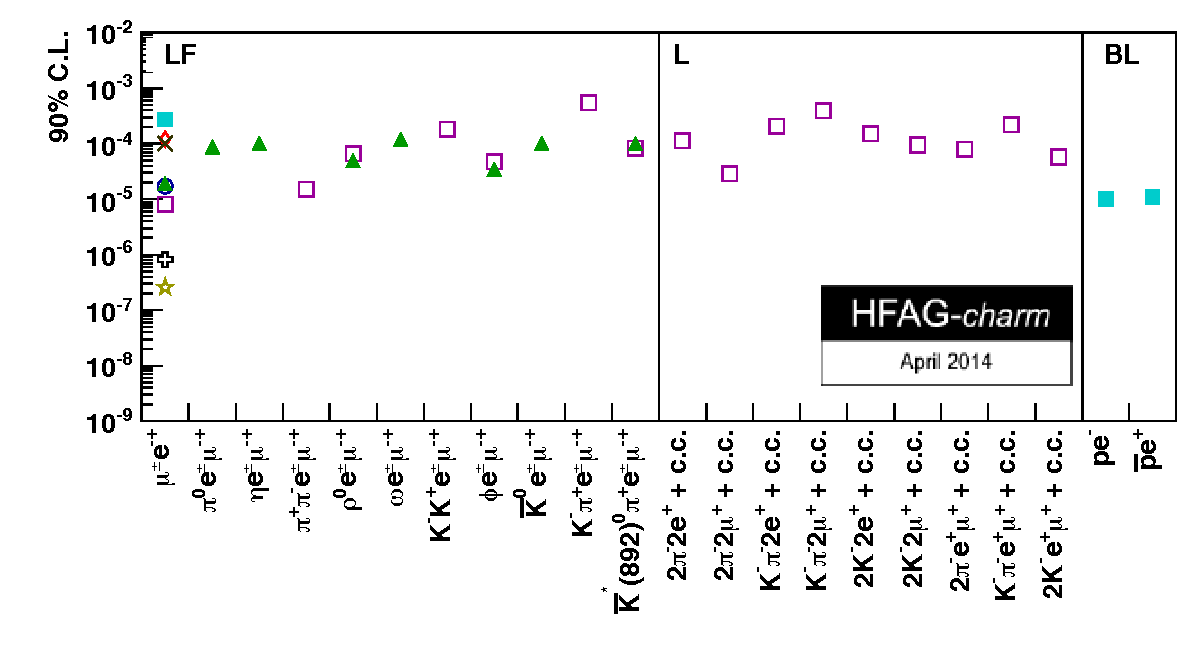
\includegraphics[width=6.0in]{figures/charm/rare_D0_2.pdf}
\caption{Upper limits at $90\%$ CL for $D^0$ decays. The top plot
shows flavor-changing neutral current decays, and the bottom plot
shows lepton-flavor-changing (LF), lepton-number-changing (L), and 
both baryon- and lepton-number-changing (BL) decays.
The legend is given in Fig.~\ref{fig:charm:lambdac}.}
\label{fig:charm:rare_d0}
\end{center}
\end{figure}

\begin{figure}
\begin{center}
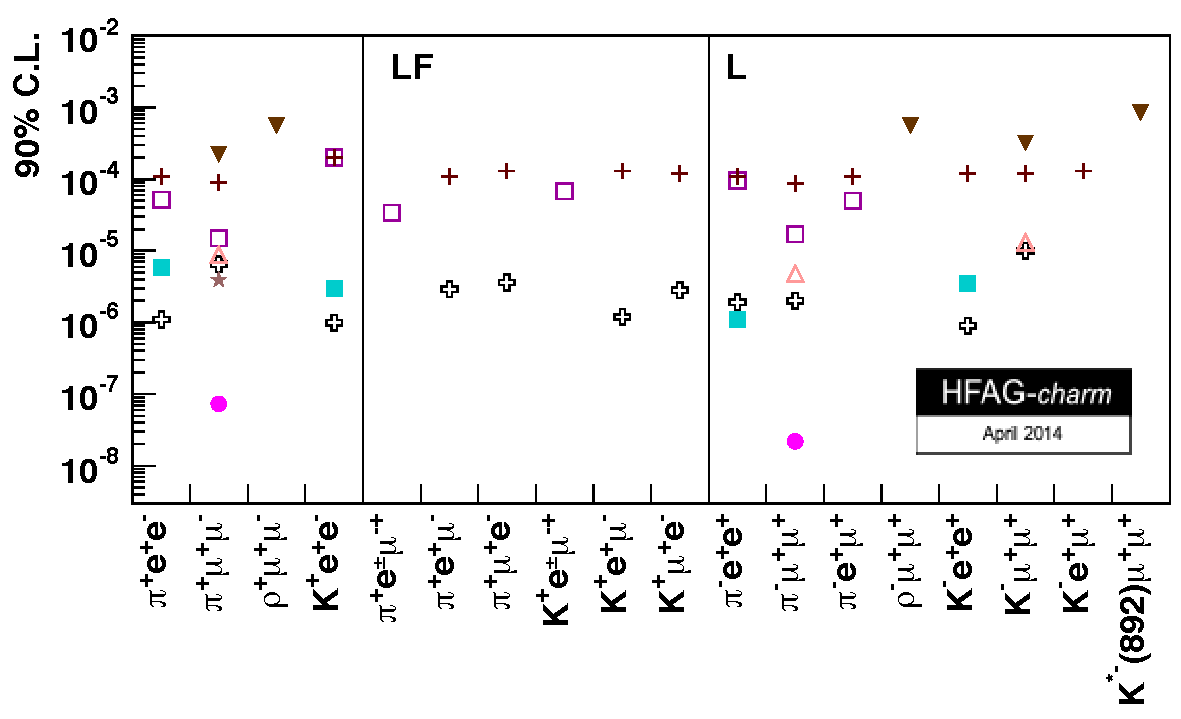
\includegraphics[width=5.0in]{figures/charm/rare_Dplus.pdf}
\vskip0.10in
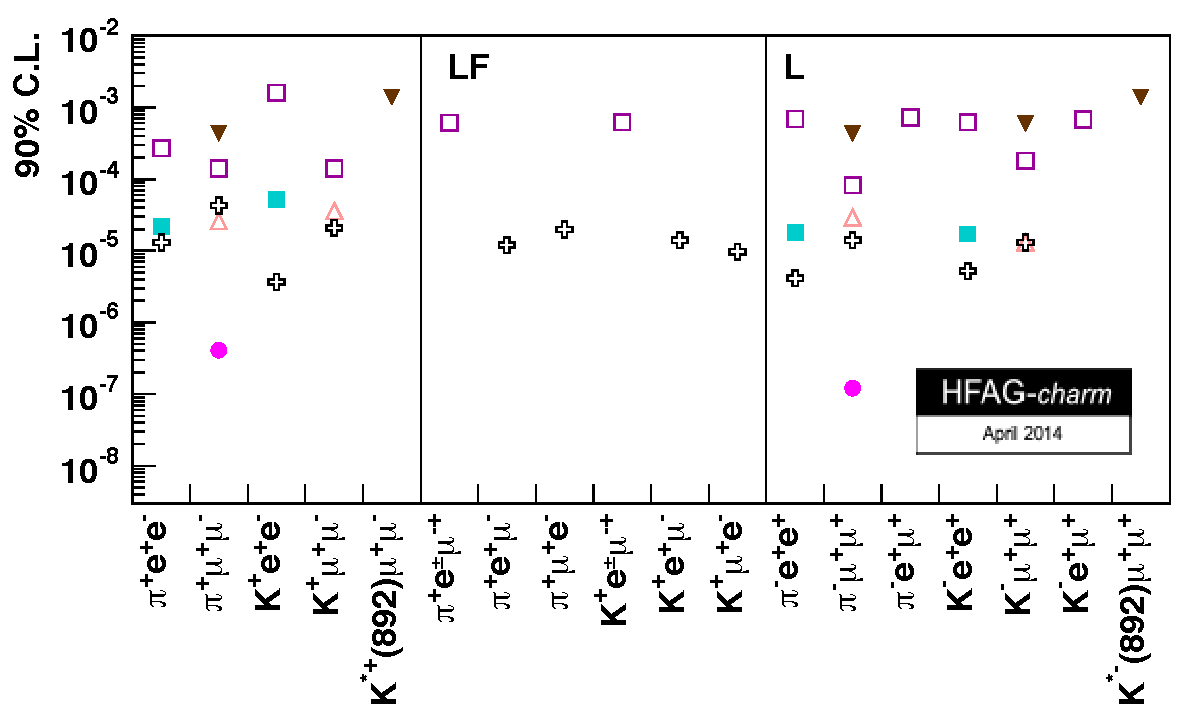
\includegraphics[width=5.0in]{figures/charm/rare_Dsplus.pdf}
\caption{Upper limits at $90\%$ CL for $D^+$ (top) and $D_s^+$ (bottom) 
decays. Each plot shows flavor-changing neutral current decays, 
lepton-flavor-changing decays (LF), and lepton-number-changing (L) decays. 
The legend is given in Fig.~\ref{fig:charm:lambdac}.}
\label{fig:charm:rare_charged}
\end{center}
\end{figure}

\begin{figure}
\begin{center}
\hbox{
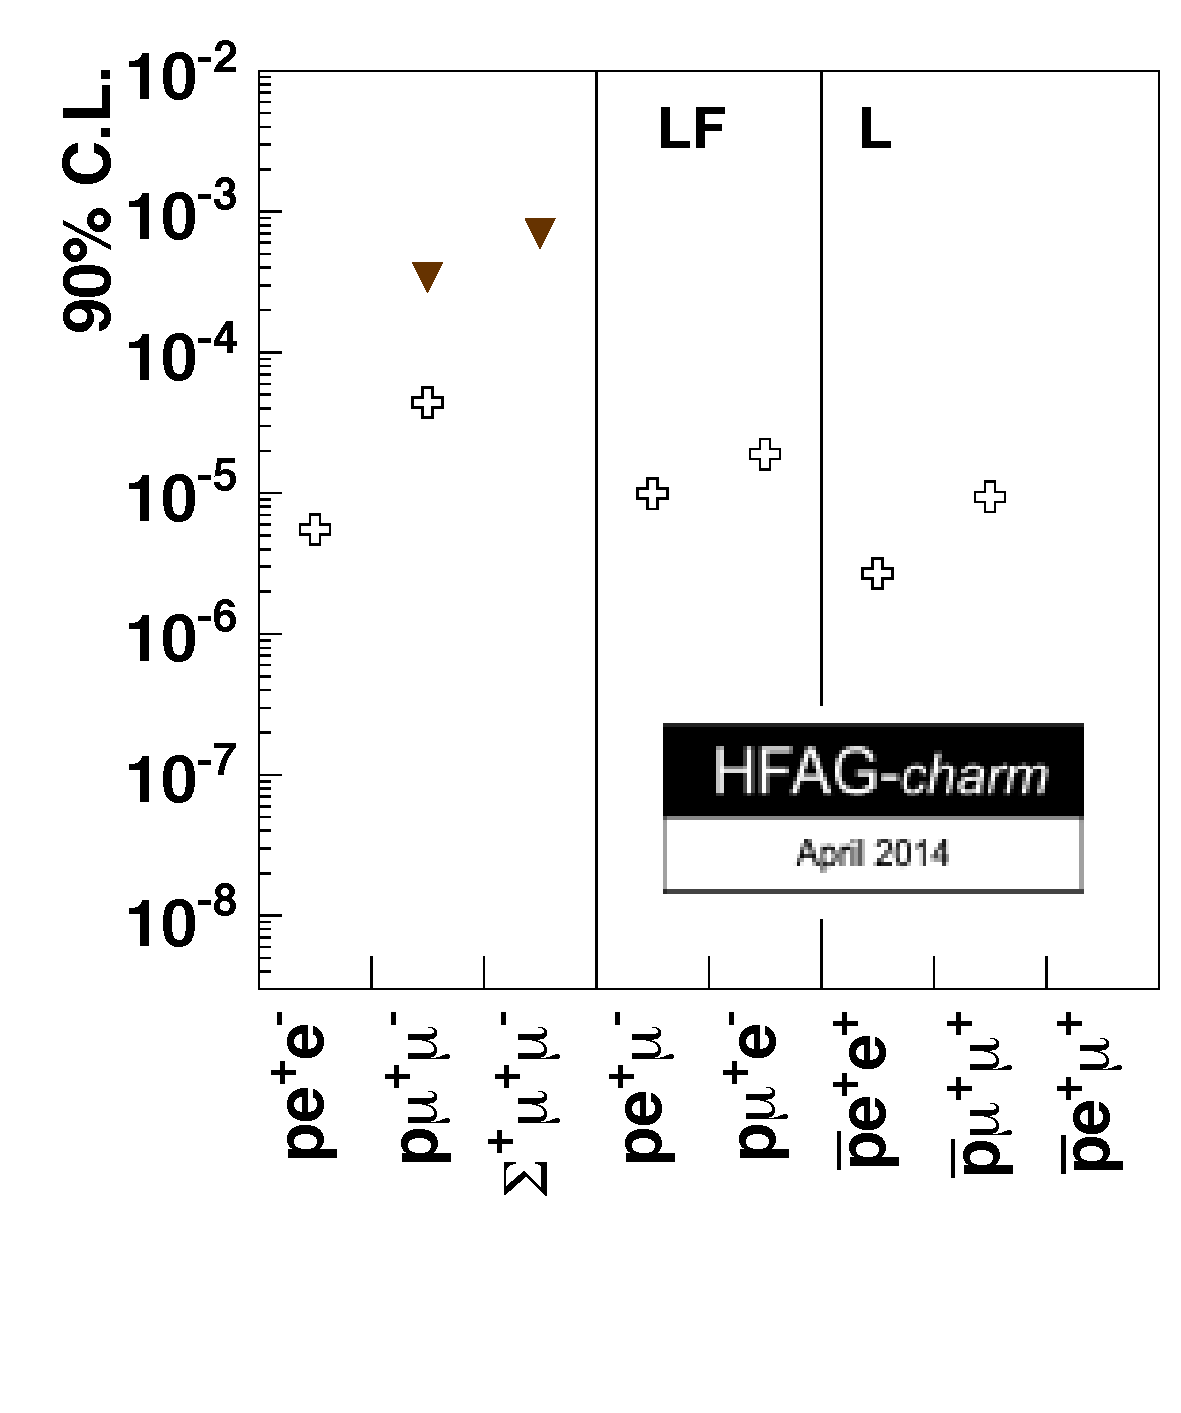
\includegraphics[width=3.0in]{figures/charm/rare_Lambdac.pdf}
\hskip-1.80in
\vbox{
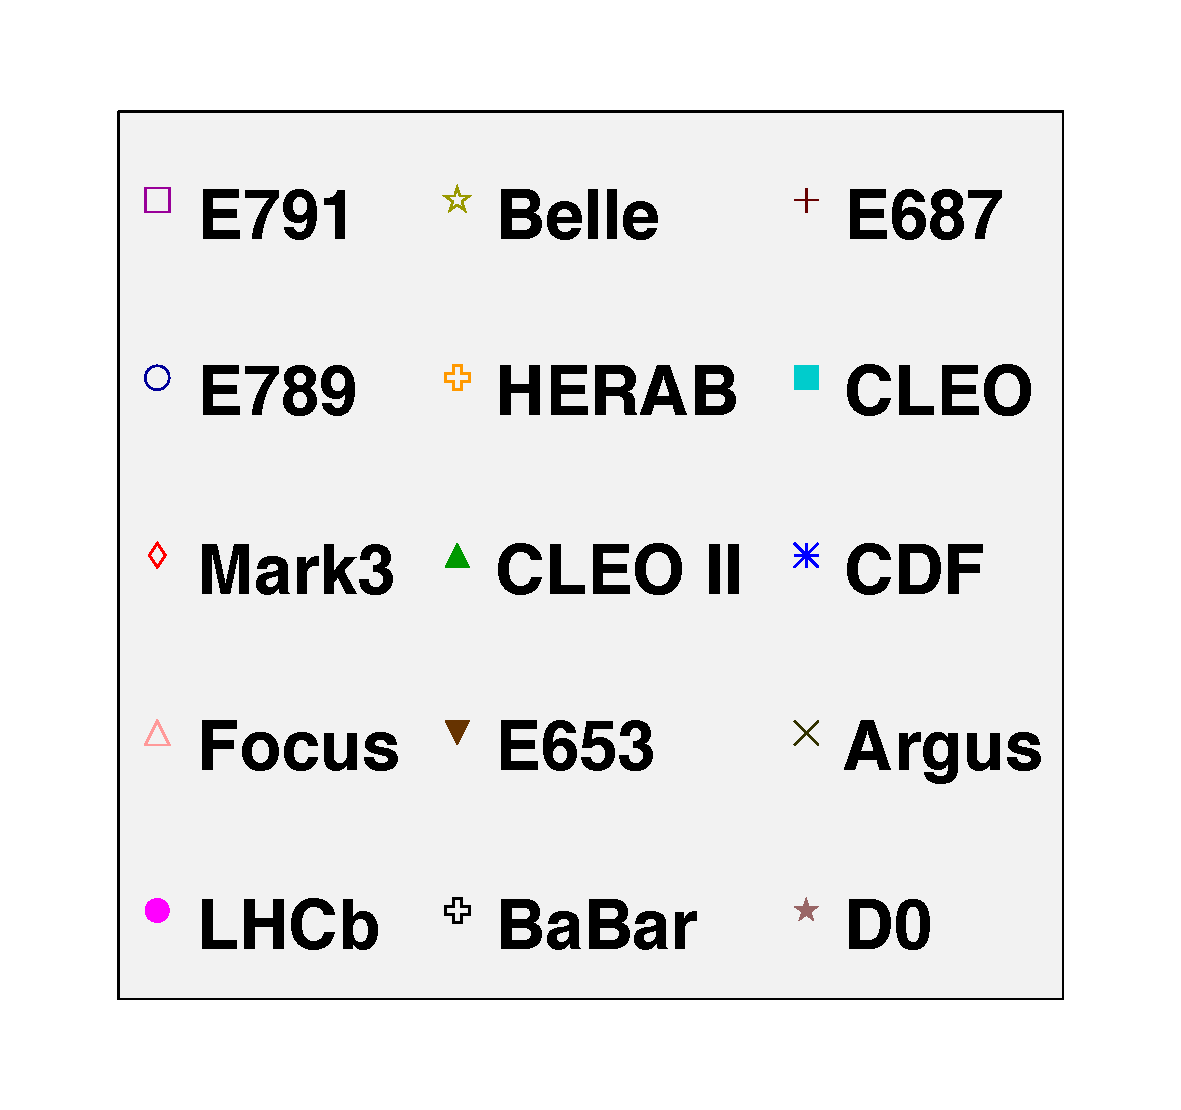
\includegraphics[width=2.5in]{figures/charm/rare_leg_all.pdf}
\vskip1.2in
}}
\vskip-0.20in
\caption{Upper limits at $90\%$ CL for $\Lambda_c^+$ decays. Shown are 
flavor-changing neutral current decays, lepton-flavor-changing (LF) 
decays, and lepton-number-changing (L) decays. }
\label{fig:charm:lambdac}
\end{center}
\end{figure}


%\begin{table}
\begin{longtable}{l|ccc}
%\centering 
\caption{Upper limits at $90\%$ CL for $D^0$ decays.%}
\label{tab:charm:rare_d0}
}\\
%\vspace{3pt}
%\begin{tabular}{l|ccc}

\hline\hline%\\
Decay & Limit $\times10^6$ & Experiment & Reference\\
\endfirsthead
% \hline\hline%\\
\multicolumn{4}{c}{\tablename\ \thetable{} -- continued from previous page} \\ \hline
Decay & Limit $\times10^6$ & Experiment & Reference\\
\endhead
\hline
$\gamma{}\gamma{}$ & 26.0 & CLEO II & \cite{Coan:2002te}\\
& 2.2 & \babar Preliminary & \cite{Lees:2011qz}\\
\hline
$e^+e^-$ & 220.0 & CLEO & \cite{Haas:1988bh}\\
& 170.0 & ARGUS & \cite{Albrecht:1988ge}\\
& 130.0 & Mark3 & \cite{Adler:1987cp}\\
& 13.0 & CLEO II & \cite{Freyberger:1996it}\\
& 8.19 & E789 & \cite{Pripstein:1999tq}\\
& 6.2 & E791 & \cite{Aitala:1999db}\\
& 1.2 & \babar & \cite{Aubert:2004bs}\\
& 0.079 & Belle & \cite{Petric:2010yt}\\
\hline
$\mu{}^+\mu{}^-$ & 70.0 & ARGUS & \cite{Albrecht:1988ge}\\
& 44.0 & E653 & \cite{Kodama:1995ia}\\
& 34.0 & CLEO II & \cite{Freyberger:1996it}\\
& 15.6 & E789 & \cite{Pripstein:1999tq}\\
& 5.2 & E791 & \cite{Aitala:1999db}\\
& 2.0 & HERAb & \cite{Abt:2004hn}\\
& 1.3 & \babar & \cite{Aubert:2004bs}\\
& 0.21 & CDF & \cite{Aaltonen:2010hz}\\
& 0.14 & Belle & \cite{Petric:2010yt}\\
& 0.0062 & LHCb & \cite{Aaij:2013cza}\\
\hline
$\pi{}^0e^+e^-$ & 45.0 & CLEO II & \cite{Freyberger:1996it}\\
\hline
$\pi{}^0\mu{}^+\mu{}^-$ & 540.0 & CLEO II & \cite{Freyberger:1996it}\\
& 180.0 & E653 & \cite{Kodama:1995ia}\\
\hline
$\eta{}e^+e^-$ & 110.0 & CLEO II & \cite{Freyberger:1996it}\\
\hline
$\eta{}\mu{}^+\mu{}^-$ & 530.0 & CLEO II & \cite{Freyberger:1996it}\\
\hline
$\pi{}^+\pi{}^-e^+e^-$ & 370.0 & E791 & \cite{Aitala:2000kk}\\
\hline
$\rho{}e^+e^-$ & 450.0 & CLEO & \cite{Haas:1988bh}\\
& 124.0 & E791 & \cite{Aitala:2000kk}\\
& 100.0 & CLEO II & \cite{Freyberger:1996it}\\
\hline
$\pi{}^+\pi{}^-\mu{}^+\mu{}^-$ & 30.0 & E791 & \cite{Aitala:2000kk}\\
& 0.55 & LHCb & \cite{Aaij:2013uoa}\\
\hline
$\rho{}\mu{}^+\mu{}^-$ & 810.0 & CLEO & \cite{Haas:1988bh}\\
& 490.0 & CLEO II & \cite{Freyberger:1996it}\\
& 230.0 & E653 & \cite{Kodama:1995ia}\\
& 22.0 & E791 & \cite{Aitala:2000kk}\\
\hline
$\omega{}e^+e^-$ & 180.0 & CLEO II & \cite{Freyberger:1996it}\\
\hline
$\omega{}\mu{}^+\mu{}^-$ & 830.0 & CLEO II & \cite{Freyberger:1996it}\\
\hline
$K^+K^-e^+e^-$ & 315.0 & E791 & \cite{Aitala:2000kk}\\
\hline
$\phi{}e^+e^-$ & 59.0 & E791 & \cite{Aitala:2000kk}\\
& 52.0 & CLEO II & \cite{Freyberger:1996it}\\
\hline
$K^+K^-\mu{}^+\mu{}^-$ & 33.0 & E791 & \cite{Aitala:2000kk}\\
\hline
$\phi{}\mu{}^+\mu{}^-$ & 410.0 & CLEO II & \cite{Freyberger:1996it}\\
& 31.0 & E791 & \cite{Aitala:2000kk}\\
\hline
$\overline{K}^0e^+e^-$ & 1700.0 & Mark3 & \cite{Adler:1988es}\\
& 110.0 & CLEO II & \cite{Freyberger:1996it}\\
\hline
$\overline{K}^0\mu{}^+\mu{}^-$ & 670.0 & CLEO II & \cite{Freyberger:1996it}\\
& 260.0 & E653 & \cite{Kodama:1995ia}\\
\hline
$K^-\pi{}^+e^+e^-$ & 385.0 & E791 & \cite{Aitala:2000kk}\\
\hline
$\overline{K}^{*0}(892)e^+e^-$ & 140.0 & CLEO II & \cite{Freyberger:1996it}\\
& 47.0 & E791 & \cite{Aitala:2000kk}\\
\hline
$K^-\pi{}^+\mu{}^+\mu{}^-$ & 360.0 & E791 & \cite{Aitala:2000kk}\\
\hline
$\overline{K}^{*0}(892)\mu{}^+\mu{}^-$ & 1180.0 & CLEO II & \cite{Freyberger:1996it}\\
& 24.0 & E791 & \cite{Aitala:2000kk}\\
\hline
$\pi{}^+\pi{}^-\pi{}^0\mu{}^+\mu{}^-$ & 810.0 & E653 & \cite{Kodama:1995ia}\\
\hline
$\mu{}^{\pm}e^{\mp}$ & 270.0 & CLEO & \cite{Haas:1988bh}\\
& 120.0 & Mark3 & \cite{Becker:1987mu}\\
& 100.0 & ARGUS & \cite{Albrecht:1988ge}\\
& 19.0 & CLEO II & \cite{Freyberger:1996it}\\
& 17.2 & E789 & \cite{Pripstein:1999tq}\\
& 8.1 & E791 & \cite{Aitala:1999db}\\
& 0.81 & \babar & \cite{Aubert:2004bs}\\
& 0.26 & Belle & \cite{Petric:2010yt}\\
\hline
$\pi{}^0e^{\pm}\mu{}^{\mp}$ & 86.0 & CLEO II & \cite{Freyberger:1996it}\\
\hline
$\eta{}e^{\pm}\mu{}^{\mp}$ & 100.0 & CLEO II & \cite{Freyberger:1996it}\\
\hline
$\pi{}^+\pi{}^-e^{\pm}\mu{}^{\mp}$ & 15.0 & E791 & \cite{Aitala:2000kk}\\
\hline
$\rho{}e^{\pm}\mu{}^{\mp}$ & 66.0 & E791 & \cite{Aitala:2000kk}\\
& 49.0 & CLEO II & \cite{Freyberger:1996it}\\
\hline
$\omega{}e^{\pm}\mu{}^{\mp}$ & 120.0 & CLEO II & \cite{Freyberger:1996it}\\
\hline
$K^+K^-e^{\pm}\mu{}^{\mp}$ & 180.0 & E791 & \cite{Aitala:2000kk}\\
\hline
$\phi{}e^{\pm}\mu{}^{\mp}$ & 47.0 & E791 & \cite{Aitala:2000kk}\\
& 34.0 & CLEO II & \cite{Freyberger:1996it}\\
\hline
$\overline{K}^0e^{\pm}\mu{}^{\mp}$ & 100.0 & CLEO II & \cite{Freyberger:1996it}\\
\hline
$K^-\pi{}^+e^{\pm}\mu{}^{\mp}$ & 550.0 & E791 & \cite{Aitala:2000kk}\\
\hline
$K^{*0}(892)e^{\pm}\mu{}^{\mp}$ & 100.0 & CLEO II & \cite{Freyberger:1996it}\\
& 83.0 & E791 & \cite{Aitala:2000kk}\\
\hline
$\pi{}^{\mp}\pi{}^{\mp}e^{\pm}e^{\pm}$ & 112.0 & E791 & \cite{Aitala:2000kk}\\
\hline
$\pi{}^{\mp}\pi{}^{\mp}\mu{}^{\pm}\mu{}^{\pm}$ & 29.0 & E791 & \cite{Aitala:2000kk}\\
\hline
$K^{\mp}\pi{}^{\mp}e^{\pm}e^{\pm}$ & 206.0 & E791 & \cite{Aitala:2000kk}\\
\hline
$K^{\mp}\pi{}^{\mp}\mu{}^{\pm}\mu{}^{\pm}$ & 390.0 & E791 & \cite{Aitala:2000kk}\\
\hline
$K^{\mp}K^{\mp}e^{\pm}e^{\pm}$ & 152.0 & E791 & \cite{Aitala:2000kk}\\
\hline
$K^{\mp}K^{\mp}\mu{}^{\pm}\mu{}^{\pm}$ & 94.0 & E791 & \cite{Aitala:2000kk}\\
\hline
$\pi{}^{\mp}\pi{}^{\mp}e^{\pm}\mu{}^{\pm}$ & 79.0 & E791 & \cite{Aitala:2000kk}\\
\hline
$K^{\mp}\pi{}^{\mp}e^{\pm}\mu{}^{\pm}$ & 218.0 & E791 & \cite{Aitala:2000kk}\\
\hline
$K^{\mp}K^{\mp}e^{\pm}\mu{}^{\pm}$ & 57.0 & E791 & \cite{Aitala:2000kk}\\
\hline
$pe^-$ & 10.0 & CLEO & \cite{Rubin:2009aa}\\
\hline
$\overline{p}e^+$ & 11.0 & CLEO & \cite{Rubin:2009aa}\\
\end{longtable}
%\end{tabular}

%\end{table}
\pagebreak

\begin{longtable}{l|ccc}
\caption{Upper limits at $90\%$ CL for $D^+$ decays.\label{tab:charm:rare_dplus}}\\
\hline\hline
Decay & Limit $\times10^6$ & Experiment & Reference\\
\endfirsthead
%\hline\hline
\multicolumn{4}{c}{\tablename\ \thetable{} -- continued from previous page} \\ \hline
Decay & Limit $\times10^6$ & Experiment & Reference\\
\endhead

\hline
$\pi{}^+e^+e^-$ & 110.0 & E687 & \cite{Frabetti:1997wp}\\
& 52.0 & E791 & \cite{Aitala:1999db}\\
& 5.9 & CLEO & \cite{Rubin:2010cq}\\
& 1.1 & \babar & \cite{Lees:2011hb}\\
\hline
$\pi{}^+\mu{}^+\mu{}^-$ & 220.0 & E653 & \cite{Kodama:1995ia}\\
& 89.0 & E687 & \cite{Frabetti:1997wp}\\
& 15.0 & E791 & \cite{Aitala:1999db}\\
& 8.8 & Focus & \cite{Link:2003qp}\\
& 6.5 & \babar & \cite{Lees:2011hb}\\
& 3.9 & D0 & \cite{Abazov:2007aj}\\
& 0.073 & LHCb & \cite{Aaij:2013sua}\\
\hline
$\rho{}^+\mu{}^+\mu{}^-$ & 560.0 & E653 & \cite{Kodama:1995ia}\\
\hline
$K^+e^+e^-$ & 200.0 & E687 & \cite{Frabetti:1997wp}\\
& 3.0 & CLEO & \cite{Rubin:2010cq}\\
& 1.0 & \babar & \cite{Lees:2011hb}\\
\hline
$\pi{}^+e^{\pm}\mu{}^{\mp}$ & 34.0 & E791 & \cite{Aitala:1999db}\\
\hline
$\pi{}^+e^+\mu{}^-$ & 110.0 & E687 & \cite{Frabetti:1997wp}\\
& 2.9 & \babar & \cite{Lees:2011hb}\\
\hline
$\pi{}^+\mu{}^+e^-$ & 130.0 & E687 & \cite{Frabetti:1997wp}\\
& 3.6 & \babar & \cite{Lees:2011hb}\\
\hline
$K^+e^{\pm}\mu{}^{\mp}$ & 68.0 & E791 & \cite{Aitala:1999db}\\
\hline
$K^+e^+\mu{}^-$ & 130.0 & E687 & \cite{Frabetti:1997wp}\\
& 1.2 & \babar & \cite{Lees:2011hb}\\
\hline
$K^+\mu{}^+e^-$ & 120.0 & E687 & \cite{Frabetti:1997wp}\\
& 2.8 & \babar & \cite{Lees:2011hb}\\
\hline
$\pi{}^-e^+e^+$ & 110.0 & E687 & \cite{Frabetti:1997wp}\\
& 96.0 & E791 & \cite{Aitala:1999db}\\
& 1.9 & \babar & \cite{Lees:2011hb}\\
& 1.1 & CLEO & \cite{Rubin:2010cq}\\
\hline
$\pi{}^-\mu{}^+\mu{}^+$ & 87.0 & E687 & \cite{Frabetti:1997wp}\\
& 17.0 & E791 & \cite{Aitala:1999db}\\
& 4.8 & Focus & \cite{Link:2003qp}\\
& 2.0 & \babar & \cite{Lees:2011hb}\\
& 0.022 & LHCb & \cite{Aaij:2013sua}\\
\hline
$\pi{}^-e^+\mu{}^+$ & 110.0 & E687 & \cite{Frabetti:1997wp}\\
& 50.0 & E791 & \cite{Aitala:1999db}\\
\hline
$\rho{}^-\mu{}^+\mu{}^+$ & 560.0 & E653 & \cite{Kodama:1995ia}\\
\hline
$K^-e^+e^+$ & 120.0 & E687 & \cite{Frabetti:1997wp}\\
& 3.5 & CLEO & \cite{Rubin:2010cq}\\
& 0.9 & \babar & \cite{Lees:2011hb}\\
\hline
$K^-\mu{}^+\mu{}^+$ & 320.0 & E653 & \cite{Kodama:1995ia}\\
& 120.0 & E687 & \cite{Frabetti:1997wp}\\
& 13.0 & Focus & \cite{Link:2003qp}\\
& 10.0 & \babar & \cite{Lees:2011hb}\\
\hline
$K^-e^+\mu{}^+$ & 130.0 & E687 & \cite{Frabetti:1997wp}\\
\hline
$K^{*-}(892)\mu{}^+\mu{}^+$ & 850.0 & E653 & \cite{Kodama:1995ia}\\

\end{longtable}

\begin{longtable}{l|ccc}
\caption{Upper limits at $90\%$ CL for $D_s^+$ decays.\label{tab:charm:rare_dsplus}}\\
\hline\hline
Decay & Limit $\times10^6$ & Experiment & Reference\\
\endfirsthead
%\hline\hline
\multicolumn{4}{c}{\tablename\ \thetable{} -- continued from previous page} \\ \hline
Decay & Limit $\times10^6$ & Experiment & Reference\\
\endhead

\hline
$\pi{}^+e^+e^-$ & 270.0 & E791 & \cite{Aitala:1999db}\\
& 22.0 & CLEO & \cite{Rubin:2010cq}\\
& 13.0 & \babar & \cite{Lees:2011hb}\\
\hline
$\pi{}^+\mu{}^+\mu{}^-$ & 430.0 & E653 & \cite{Kodama:1995ia}\\
& 140.0 & E791 & \cite{Aitala:1999db}\\
& 43.0 & \babar & \cite{Lees:2011hb}\\
& 26.0 & Focus & \cite{Link:2003qp}\\
& 0.41 & LHCb & \cite{Aaij:2013sua}\\
\hline
$K^+e^+e^-$ & 1600.0 & E791 & \cite{Aitala:1999db}\\
& 52.0 & CLEO & \cite{Rubin:2010cq}\\
& 3.7 & \babar & \cite{Lees:2011hb}\\
\hline
$K^+\mu{}^+\mu{}^-$ & 140.0 & E791 & \cite{Aitala:1999db}\\
& 36.0 & Focus & \cite{Link:2003qp}\\
& 21.0 & \babar & \cite{Lees:2011hb}\\
\hline
$K^{*+}(892)\mu{}^+\mu{}^-$ & 1400.0 & E653 & \cite{Kodama:1995ia}\\
\hline
$\pi{}^+e^{\pm}\mu{}^{\mp}$ & 610.0 & E791 & \cite{Aitala:1999db}\\
\hline
$\pi{}^+e^+\mu{}^-$ & 12.0 & \babar & \cite{Lees:2011hb}\\
\hline
$\pi{}^+\mu{}^+e^-$ & 20.0 & \babar & \cite{Lees:2011hb}\\
\hline
$K^+e^{\pm}\mu{}^{\mp}$ & 630.0 & E791 & \cite{Aitala:1999db}\\
\hline
$K^+e^+\mu{}^-$ & 14.0 & \babar & \cite{Lees:2011hb}\\
\hline
$K^+\mu{}^+e^-$ & 9.7 & \babar & \cite{Lees:2011hb}\\
\hline
$\pi{}^-e^+e^+$ & 690.0 & E791 & \cite{Aitala:1999db}\\
& 18.0 & CLEO & \cite{Rubin:2010cq}\\
& 4.1 & \babar & \cite{Lees:2011hb}\\
\hline
$\pi{}^-\mu{}^+\mu{}^+$ & 430.0 & E653 & \cite{Kodama:1995ia}\\
& 82.0 & E791 & \cite{Aitala:1999db}\\
& 29.0 & Focus & \cite{Link:2003qp}\\
& 14.0 & \babar & \cite{Lees:2011hb}\\
& 0.12 & LHCb & \cite{Aaij:2013sua}\\
\hline
$\pi{}^-e^+\mu{}^+$ & 730.0 & E791 & \cite{Aitala:1999db}\\
\hline
$K^-e^+e^+$ & 630.0 & E791 & \cite{Aitala:1999db}\\
& 17.0 & CLEO & \cite{Rubin:2010cq}\\
& 5.2 & \babar & \cite{Lees:2011hb}\\
\hline
$K^-\mu{}^+\mu{}^+$ & 590.0 & E653 & \cite{Kodama:1995ia}\\
& 180.0 & E791 & \cite{Aitala:1999db}\\
& 13.0 & \babar & \cite{Lees:2011hb}\\
\hline
$K^-e^+\mu{}^+$ & 680.0 & E791 & \cite{Aitala:1999db}\\
\hline
$K^{*-}(892)\mu{}^+\mu{}^+$ & 1400.0 & E653 & \cite{Kodama:1995ia}\\

\end{longtable}

\begin{longtable}{l|ccc}
\caption{Upper limits at $90\%$ CL for $\Lambda_c^+$ decays.\label{tab:charm:rare_lambdac}}\\
\hline\hline
Decay & Limit $\times10^6$ & Experiment & Reference\\
\endfirsthead
%\hline\hline
\multicolumn{4}{c}{\tablename\ \thetable{} -- continued from previous page} \\ \hline
Decay & Limit $\times10^6$ & Experiment & Reference\\
\endhead

\hline
$pe^+e^-$ & 5.5 & \babar & \cite{Lees:2011hb}\\
\hline
$p\mu{}^+\mu{}^-$ & 340.0 & E653 & \cite{Kodama:1995ia}\\
& 44.0 & \babar & \cite{Lees:2011hb}\\
\hline
$\sigma{}^+\mu{}^+\mu{}^-$ & 700.0 & E653 & \cite{Kodama:1995ia}\\
\hline
$pe^+\mu{}^-$ & 9.9 & \babar & \cite{Lees:2011hb}\\
\hline
$p\mu{}^+e^-$ & 19.0 & \babar & \cite{Lees:2011hb}\\
\hline
$\overline{p}e^+e^+$ & 2.7 & \babar & \cite{Lees:2011hb}\\
\hline
$\overline{p}\mu{}^+\mu{}^+$ & 9.4 & \babar & \cite{Lees:2011hb}\\

\end{longtable}
